\documentclass[11pt,a4paper]{article}

% Configuración de página y márgenes
\usepackage[margin=1in, top=1.2in, bottom=1.2in]{geometry}

% Paquetes para caracteres especiales y codificación
\usepackage[utf8]{inputenc}
\usepackage[T1]{fontenc}
\usepackage{lmodern}

% Soporte para idiomas (español e inglés)
\usepackage[spanish,english]{babel}

% Paquetes para imágenes y gráficos
\usepackage{graphicx}
\usepackage{float}
\usepackage{caption}
\usepackage{subcaption}

% Paquetes para tablas
\usepackage{longtable}
\usepackage{booktabs}
\usepackage{array}
\usepackage{multirow}
\usepackage{multicol}
\usepackage{tabularx}

% Control de saltos de página
\usepackage{needspace}
\usepackage{afterpage}
\usepackage{placeins}

% Enlaces e hipervínculos
\usepackage[colorlinks=true, linkcolor=blue, urlcolor=blue, citecolor=blue]{hyperref}

% Paquetes para código y verbatim
\usepackage{fancyvrb}
\usepackage{listings}
\usepackage{xcolor}

% Configuración de listings para código
\lstset{
    basicstyle=\ttfamily\small,
    breaklines=true,
    frame=single,
    backgroundcolor=\color{gray!10},
    keywordstyle=\color{blue},
    commentstyle=\color{green!50!black},
    stringstyle=\color{red}
}

% Paquetes para mejor tipografía
\usepackage{microtype}
\usepackage{setspace}

% Configuración de espaciado
\onehalfspacing

% Comandos personalizados
\providecommand{\tightlist}{}

% Comando para evitar viudas y huérfanas
\widowpenalty=10000
\clubpenalty=10000

% Configuración de profundidad de numeración
\setcounter{secnumdepth}{3}
\setcounter{tocdepth}{3}

\begin{document}


    
    % Título principal
    {\Huge \textbf{Hoja de Datos del Módulo DevLab}}\\[1.5em]
    
    % Subtítulo si existe
    
    
    % Autor
    
    
    % Fecha
    
    
    \vfill
    
    % Información adicional al pie
    
    
    
\end{titlepage}

% Tabla de contenidos


% Lista de figuras (si hay imágenes)


% Lista de tablas (si hay tablas)




% Contenido principal del documento
\section{Documentación de Hardware}

\subsection{Descripción General}

El módulo sensor de presión barométrica ICP-10111 es un sensor ambiental compacto con capacidades integradas de monitoreo ambiental, diseñado para aplicaciones IoT y mediciones atmosféricas precisas.

\subsection{Características Principales}

\begin{itemize}
\item \textbf{Sensor de presión ICP-10111} (Alta precisión)
\item \textbf{Sensor ambiental BME688} (Temperatura, humedad, gas)
\item \textbf{Modos de bajo consumo} energético
\item \textbf{Conectividad I2C/QWIIC}
\item \textbf{Factor de forma compacto} con orificios castellanos
\end{itemize}

\section{Hardware}

\subsection{Technical Specifications Especificaciones Técnicas}

\subsubsection{Especificaciones del Sensor}


\begin{table}[H]
\centering
\small
\begin{tabular}{|l|l|l|l|}
\hline
Parámetro & Valor & Unidad & Notas \\
\hline
Rango de Presión & 300-1250 & hPa & Presión absoluta \\
Precisión de Presión & $\pm$0.4 & hPa & A 25$^{\circ}$C \\
Rango de Temperatura & -40 a +85 & $^{\circ}$C & Rango de operación \\
Rango de Humedad & 0-100 & %RH & Humedad relativa \\
Interfaz & I2C & - & Compatible QWIIC \\
\hline
\end{tabular}
\caption{Especificaciones técnicas}
\end{table}


\subsubsection{Especificaciones de Alimentación}


\begin{table}[H]
\centering
\small
\begin{tabular}{|l|l|l|l|l|l|}
\hline
Parámetro & Mín & Típ & Máx & Unidad & Condiciones \\
\hline
Voltaje de Alimentación & 3.0 & 3.3 & 5.0 & V & Operación Normal \\
Corriente Activa & - & 1.2 & 2.0 & mA & Medición continua \\
Corriente en Reposo & - & 0.1 & 0.5 & $\mu$A & Modo standby \\
Salida del Regulador & - & 1.8 & - & V & LDO interno \\
\hline
\end{tabular}
\caption{Especificaciones técnicas}
\end{table}


\subsection{Pinout Distribución de Pines}


\begin{figure}[H]
\centering
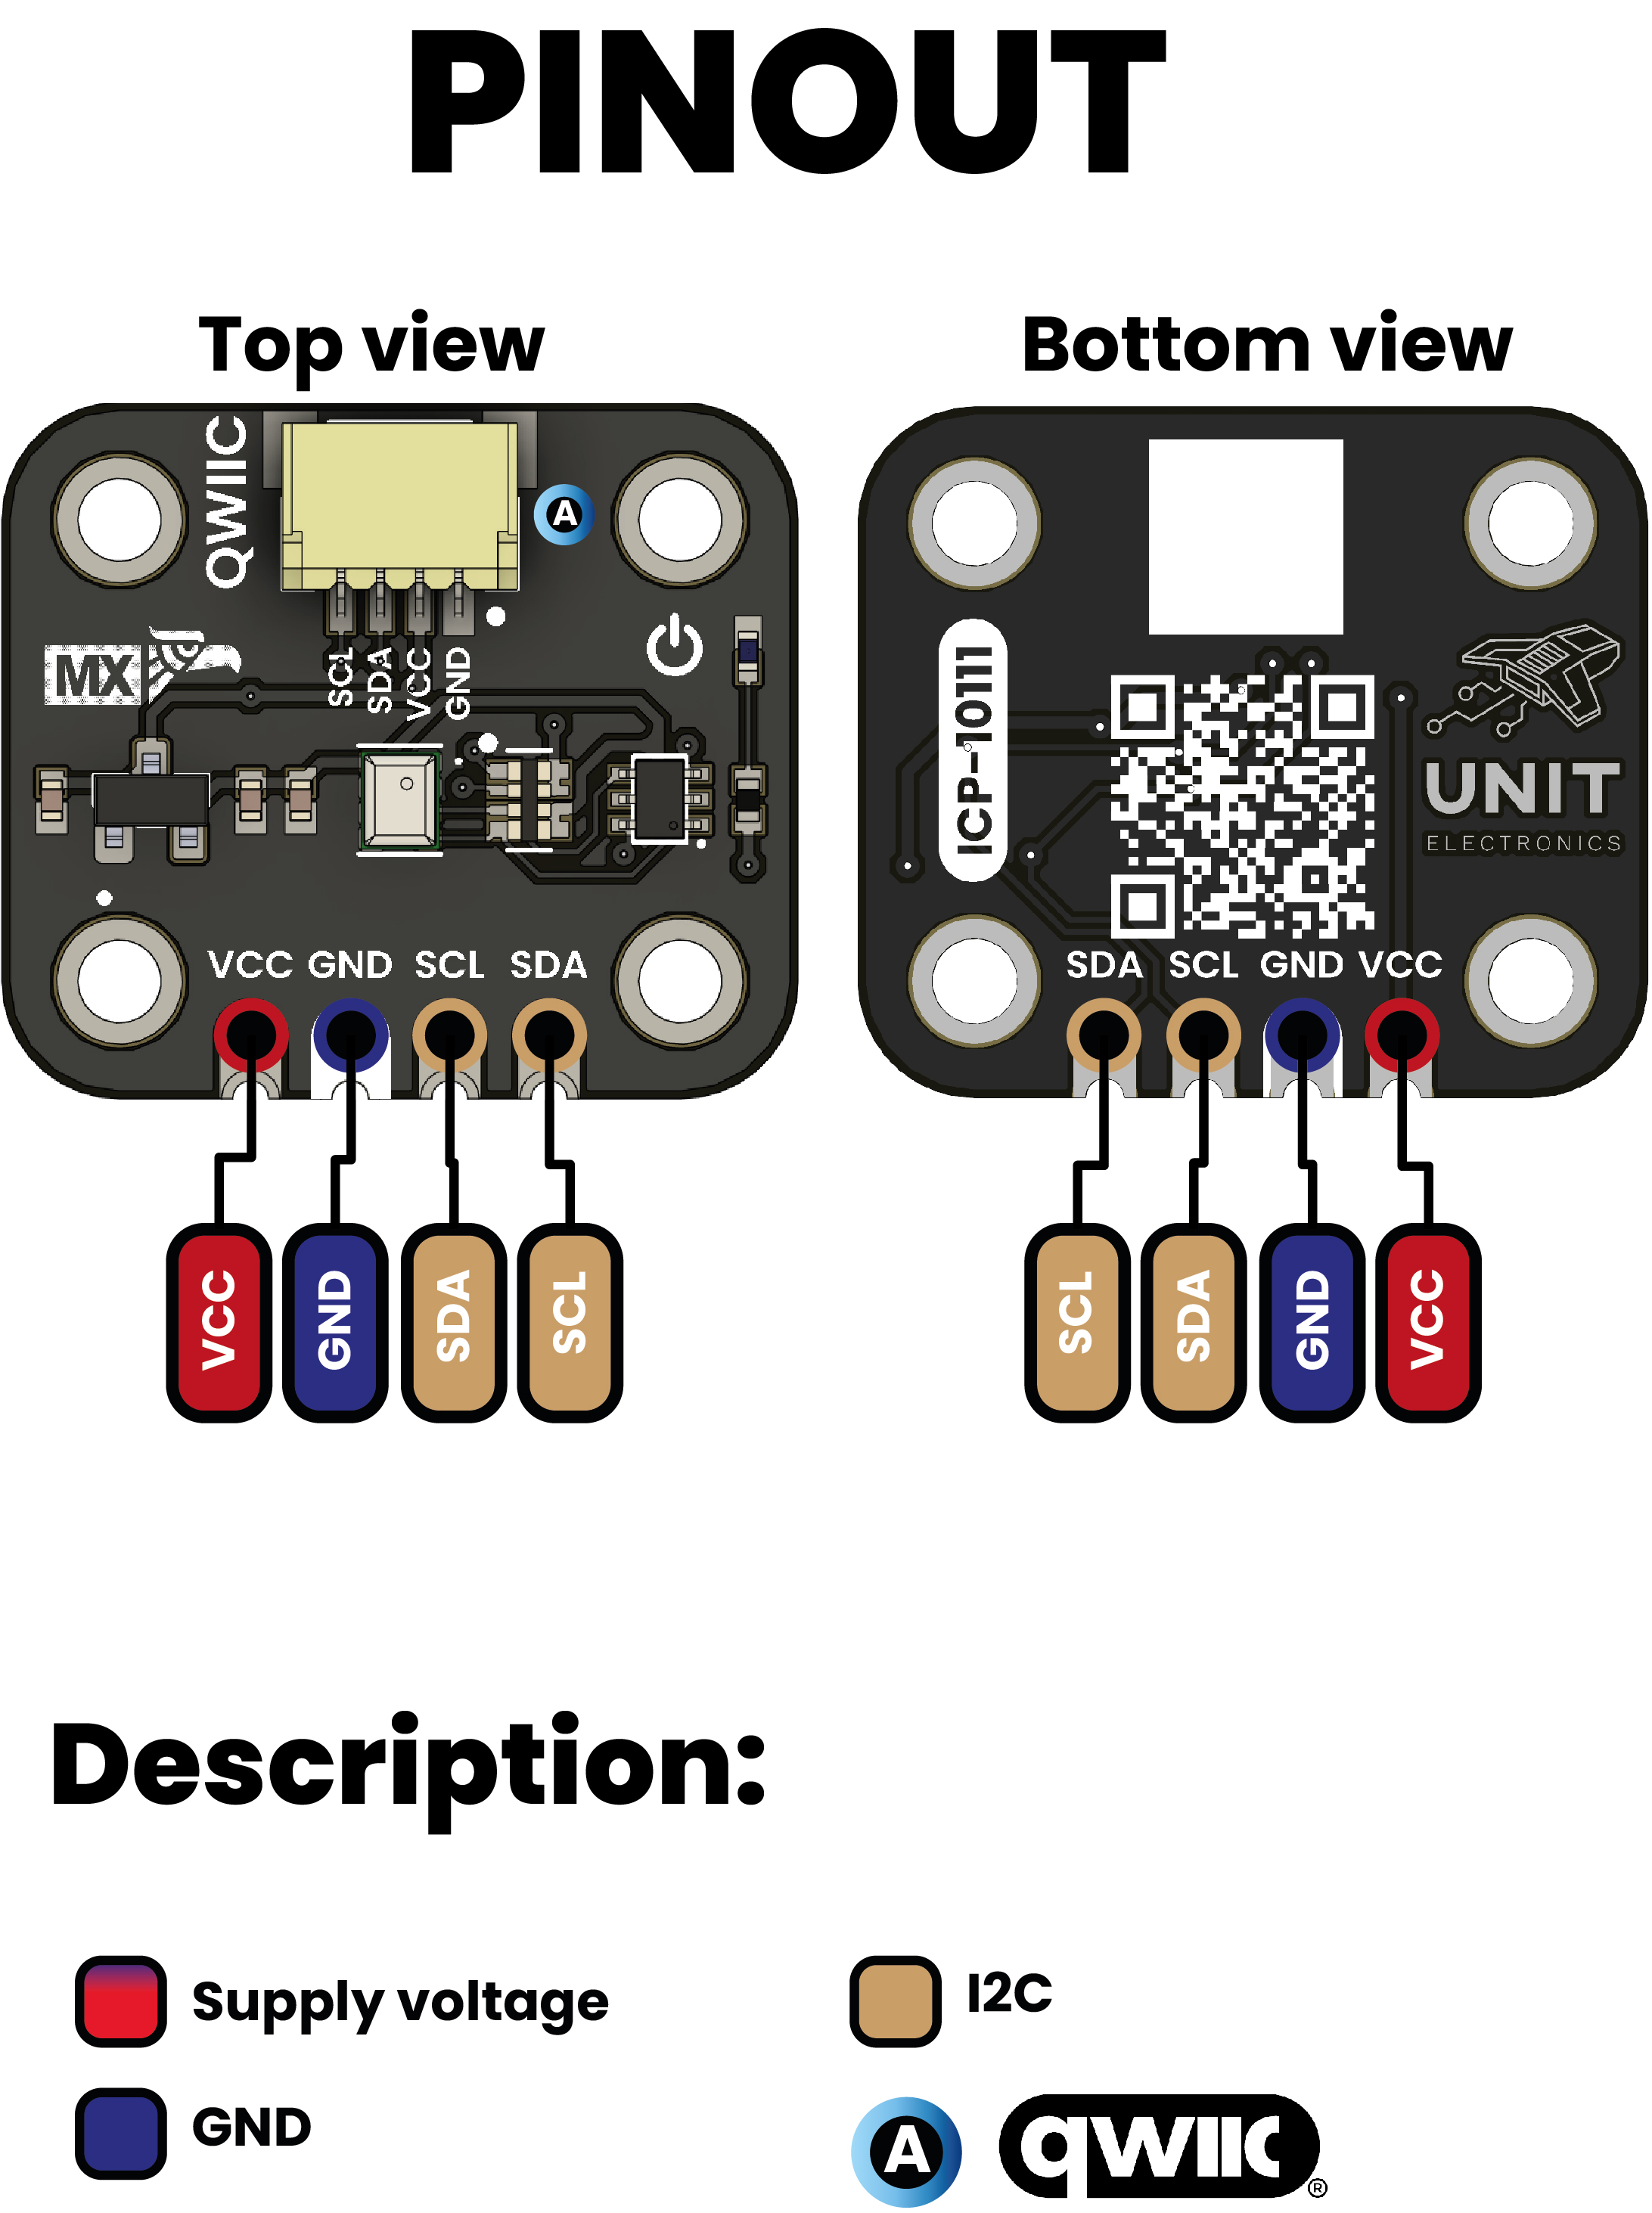
\includegraphics[width=0.9\textwidth]{es_unit_pinout_v_0_0_1_ue0094_icp10111_barometric_pressure_sensor_en.jpg}
\caption{Diagrama de Pines}
\label{fig:es-unit-pinout-v-0-0-1-ue0094-icp10111-barometric-pressure-sensor-en-jpg}
\end{figure}




\begin{table}[H]
\centering
\small
\begin{tabular}{|c|c|c|}
\hline
Etiqueta & Función & Notas \\
\hline
VCC & Alimentación & 3.3V o 5V \\
GND & Tierra & Tierra común para todos los componentes \\
SDA & Datos I2C & Línea de datos serie \\
SCL & Reloj I2C & Línea de reloj serie \\
\hline
\end{tabular}
\caption{Especificaciones técnicas}
\end{table}


\subsection{Dimensions Dimensiones}


\begin{figure}[H]
\centering
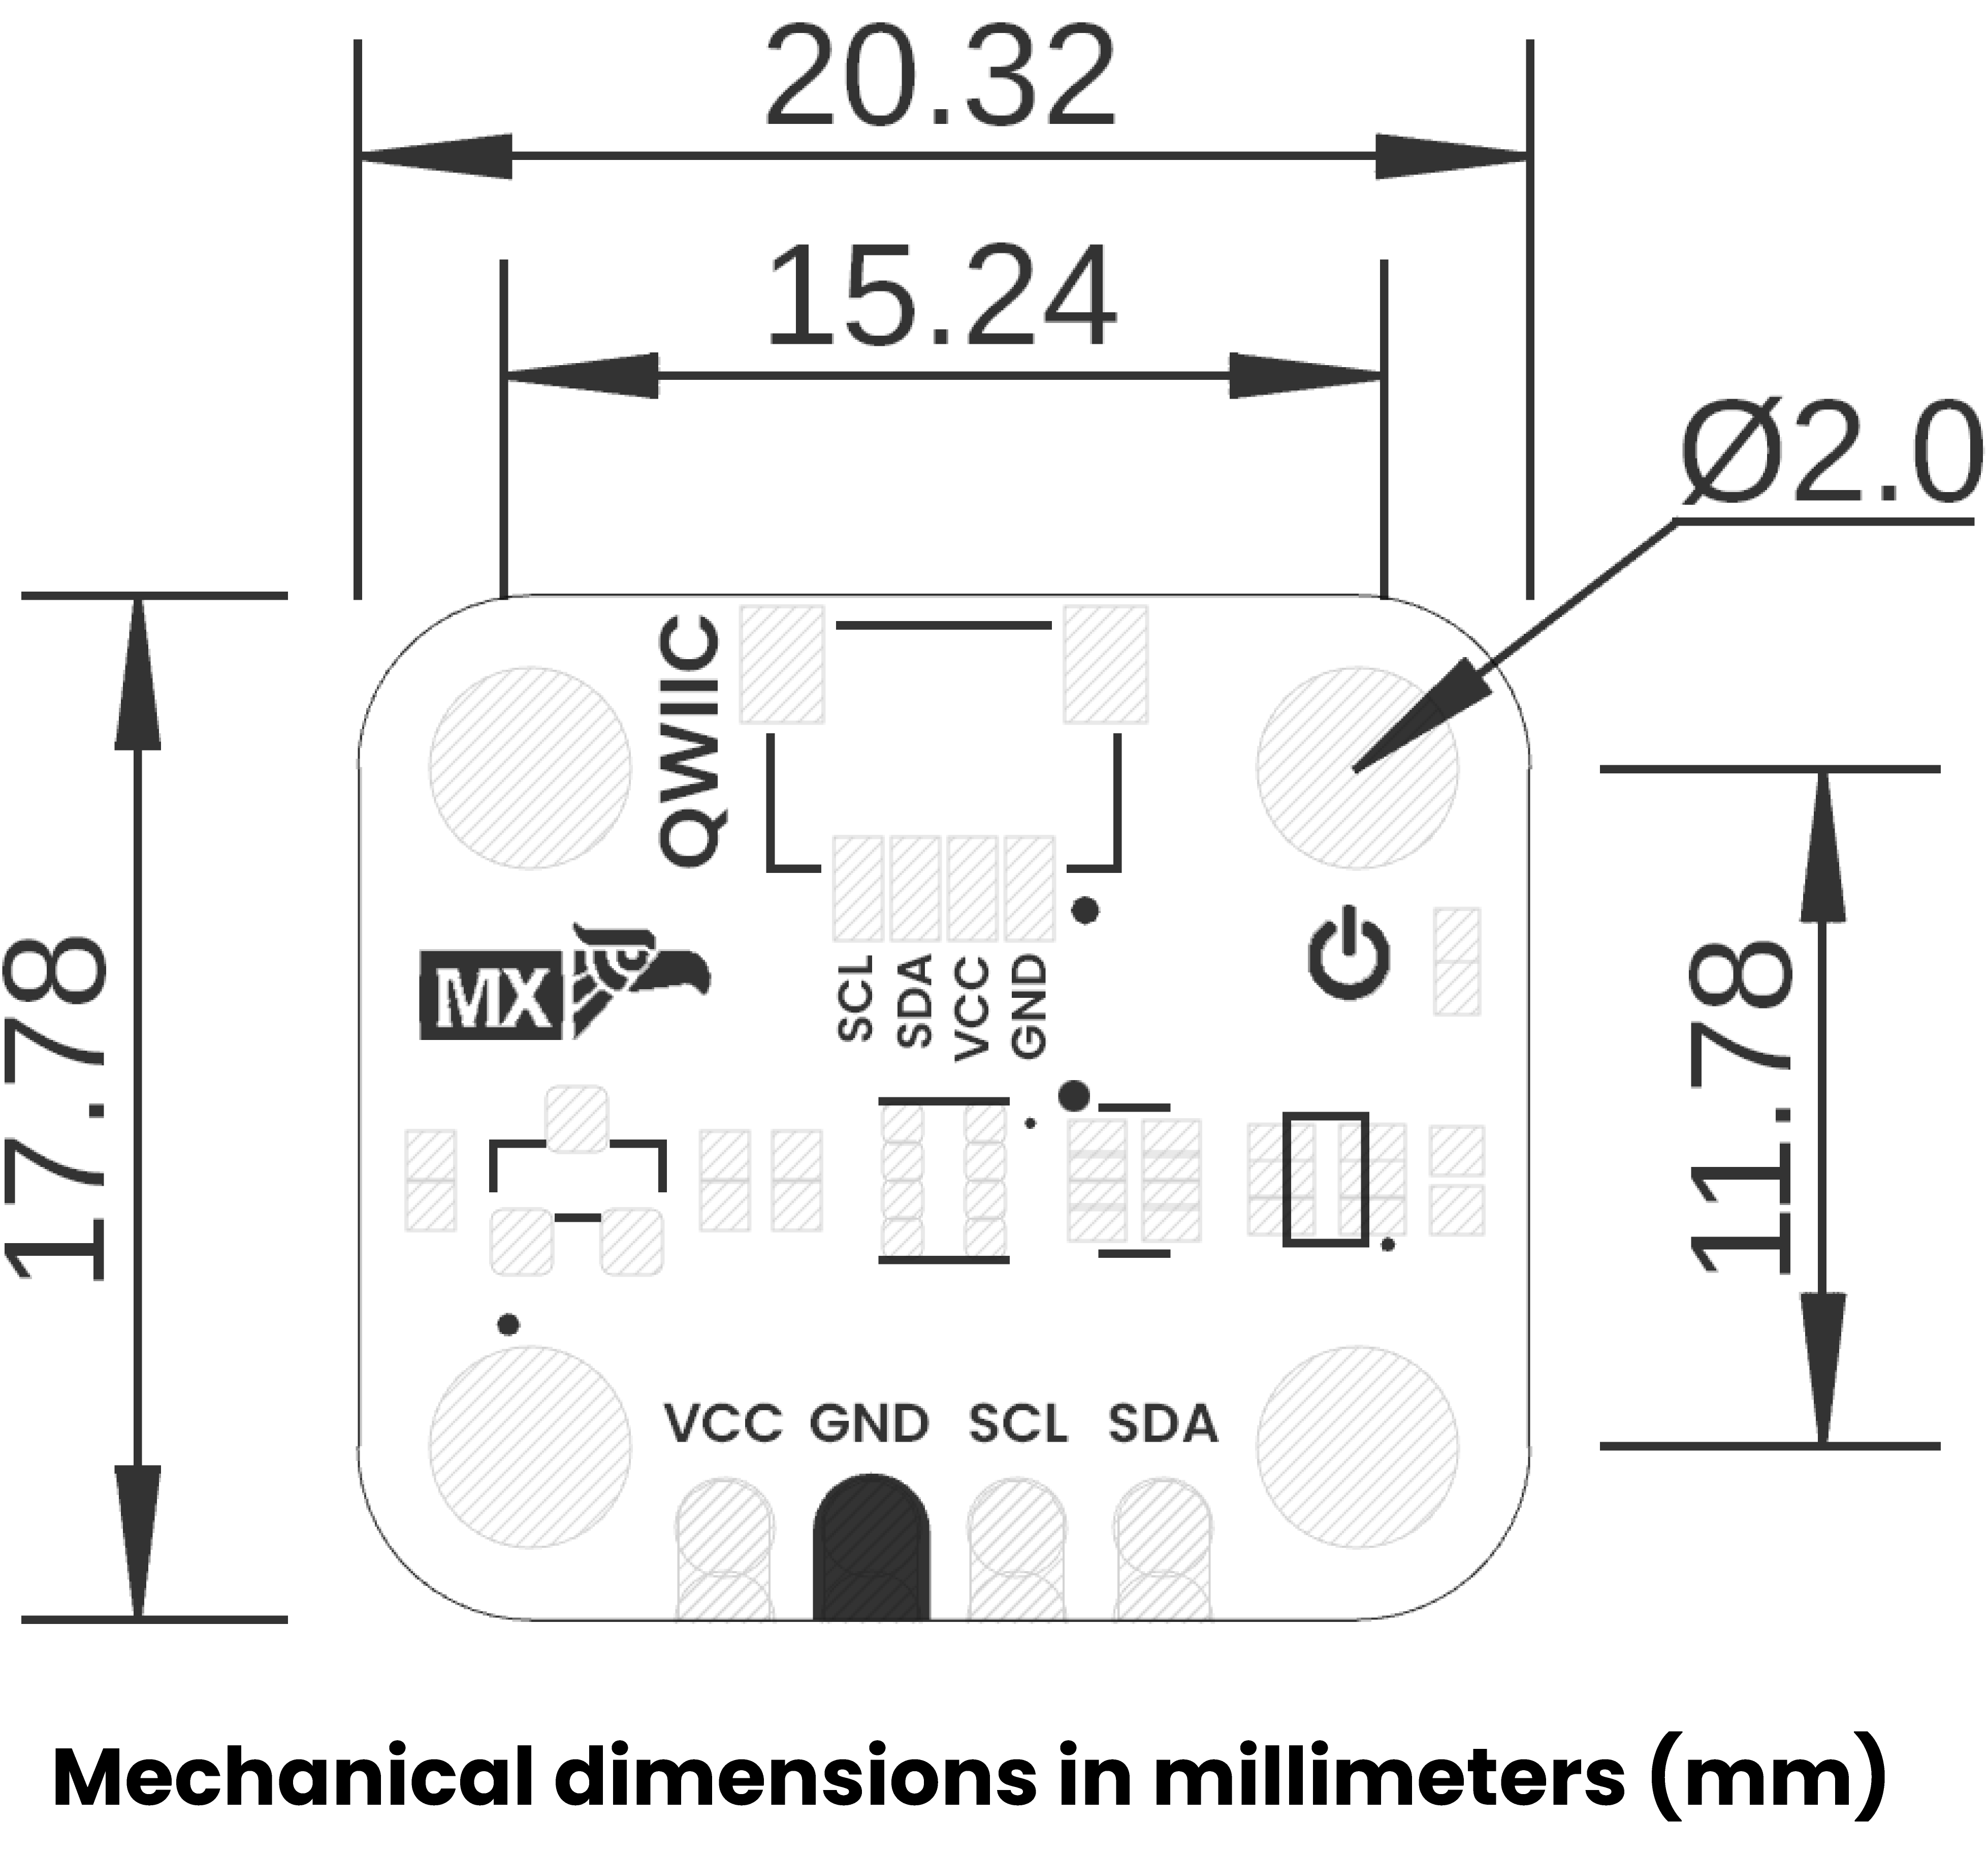
\includegraphics[width=0.6\textwidth]{es_unit_dimension_v_1_0_0_icp10111_barometric_pressure_sensor.png}
\caption{Dimensiones}
\label{fig:es-unit-dimension-v-1-0-0-icp10111-barometric-pressure-sensor-png}
\end{figure}



\subsection{Topology Topología}


\begin{figure}[H]
\centering
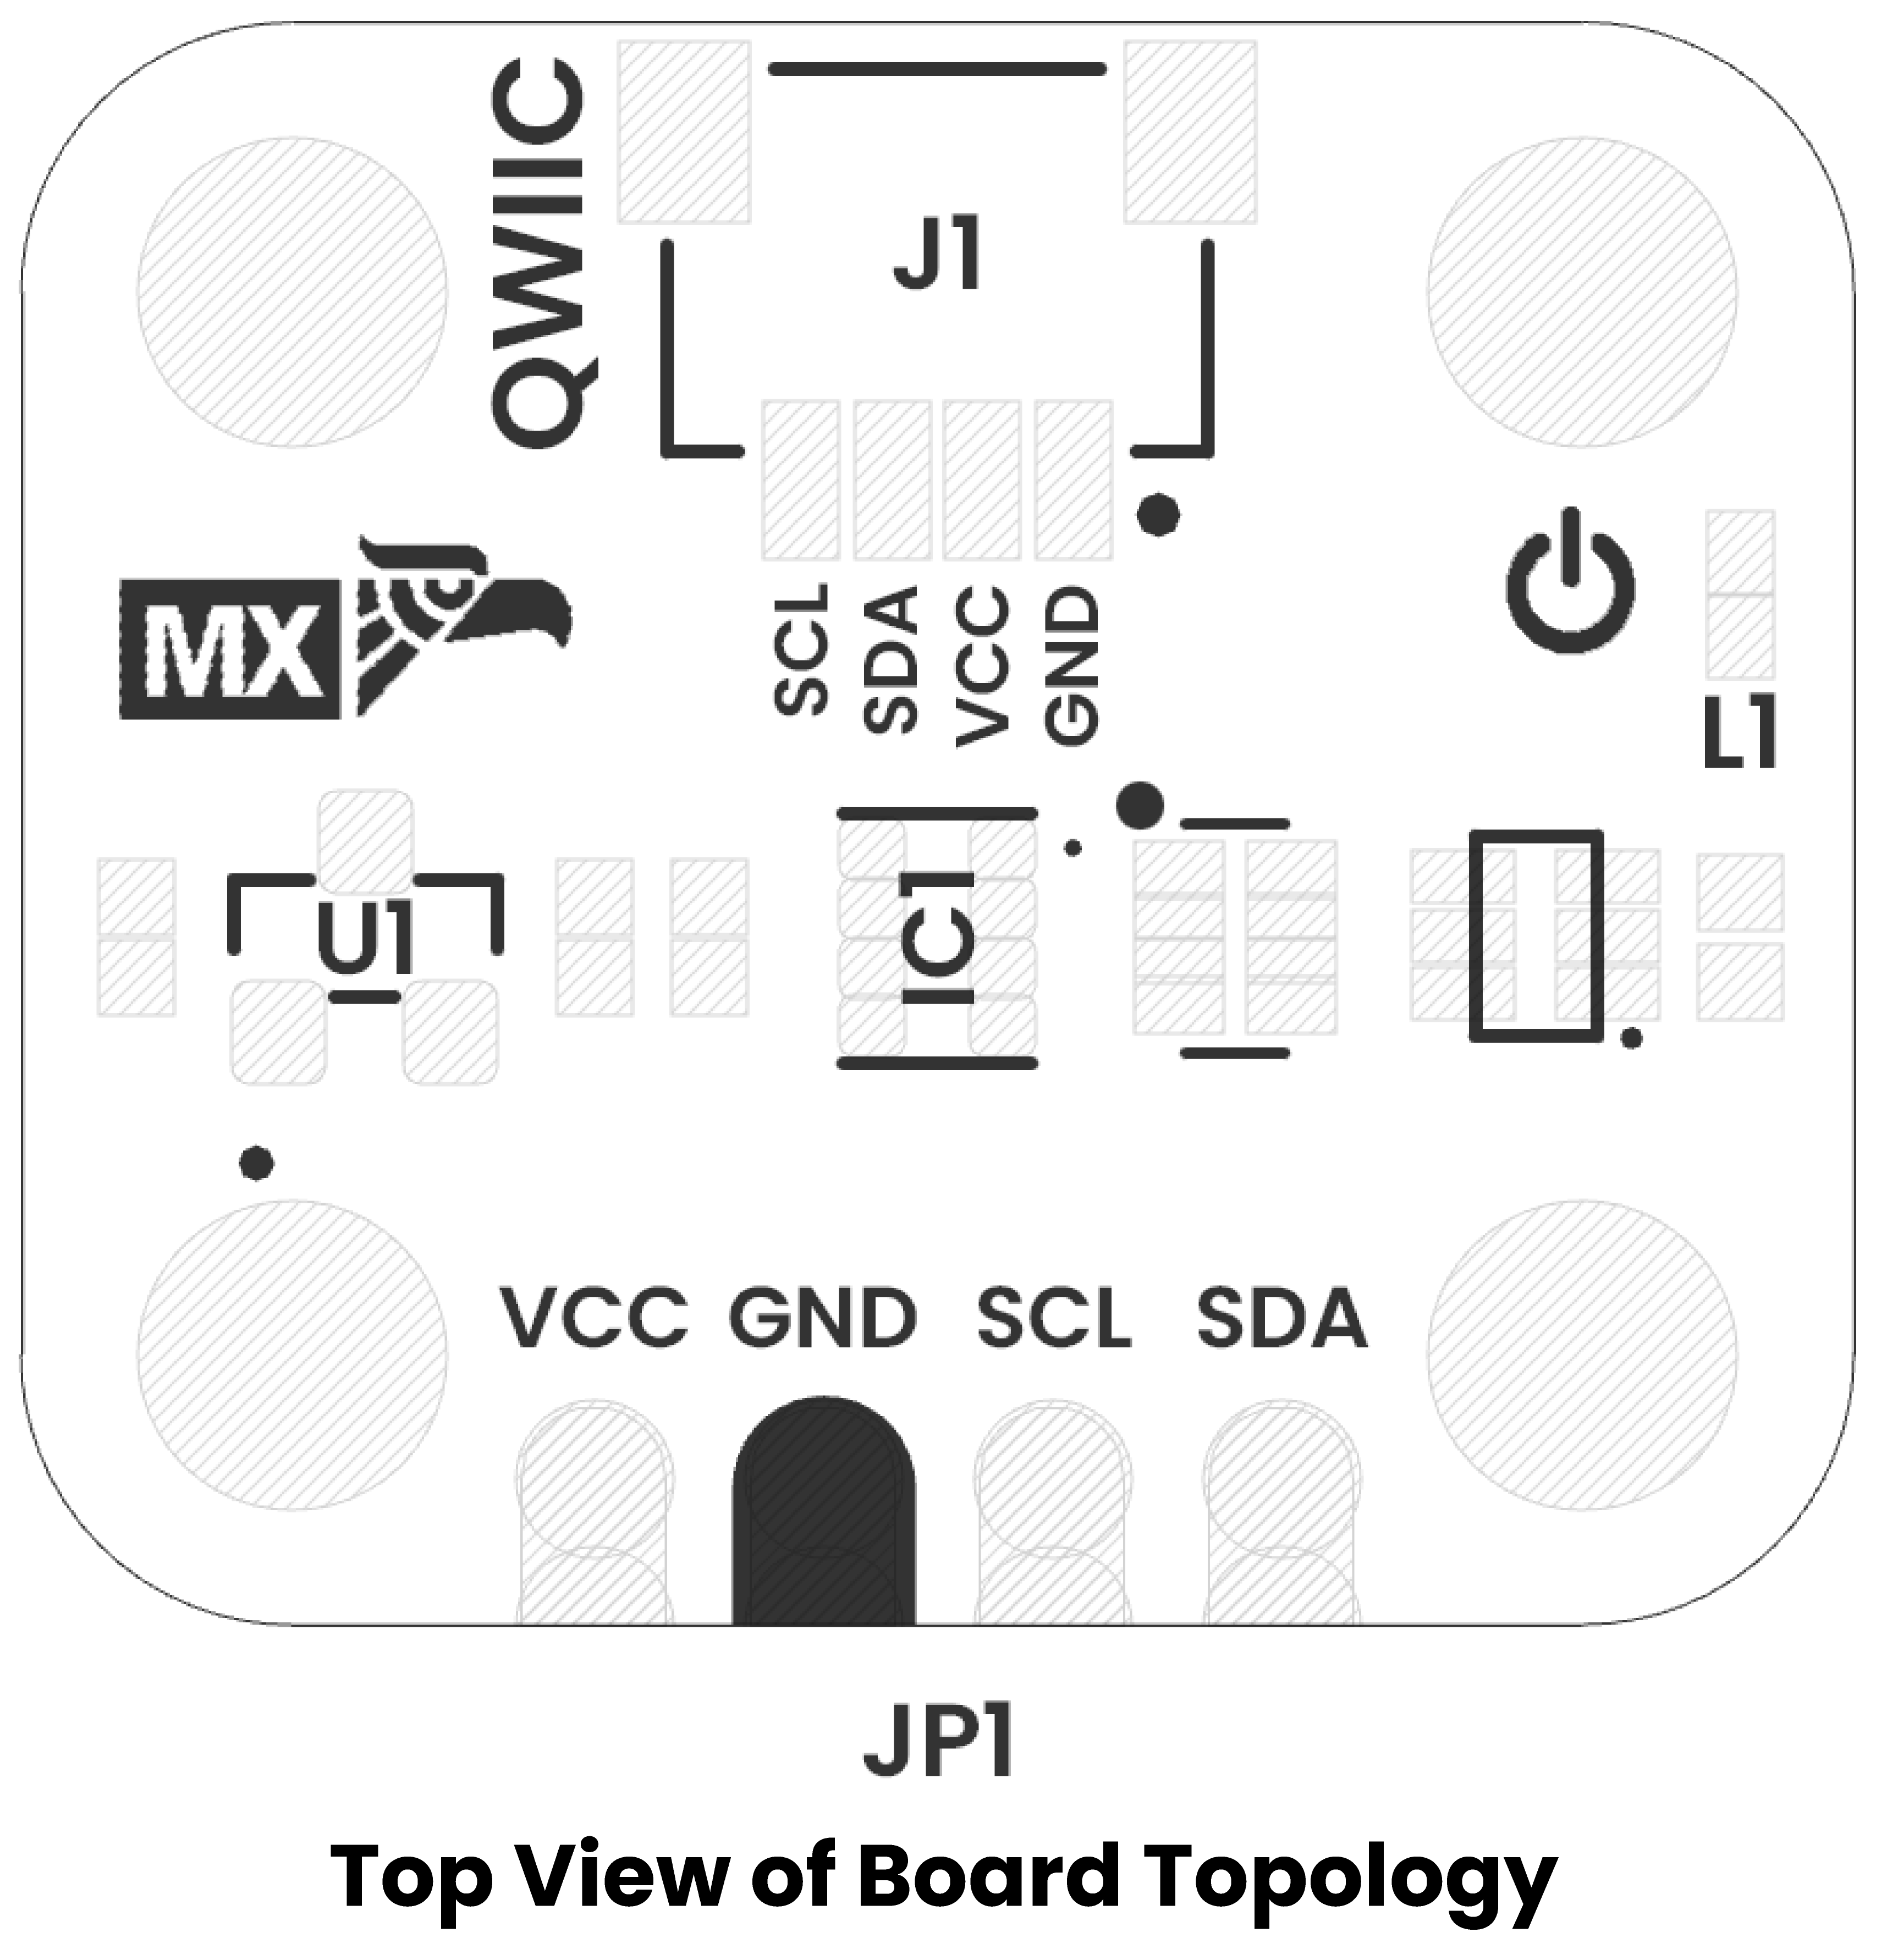
\includegraphics[width=0.7\textwidth]{es_unit_topology_v_1_0_0_icp10111_barometric_pressure_sensor.png}
\caption{Topología}
\label{fig:es-unit-topology-v-1-0-0-icp10111-barometric-pressure-sensor-png}
\end{figure}




\begin{table}[H]
\centering
\small
\begin{tabular}{|c|c|}
\hline
Ref. & Descripción \\
\hline
IC1 & Sensor de Presión Barométrica ICP-10111 \\
IC2 & Sensor Ambiental BME688 \\
L1 & LED de Encendido \\
U1 & Regulador ME6206A18XG 1.8V \\
JP1 & Orificios Castellanos de 2.54 mm \\
J1 & Conector QWIIC (JST paso 1 mm) para I2C \\
\hline
\end{tabular}
\caption{Especificaciones técnicas}
\end{table}


\subsection{Interfaces de Comunicación}

\subsubsection{Interfaz I2C}
\begin{itemize}
\item \textbf{Dirección}: 0x63 (ICP-10111), 0x77 (BME688)
\item \textbf{Velocidad}: Estándar (100 kHz), Rápido (400 kHz)
\item \textbf{Características}: Conector compatible QWIIC
\item \textbf{Resistencias Pull-up}: 4.7k$\Omega$ integradas
\end{itemize}

\subsubsection{Especificaciones de Interfaz Digital}
\begin{itemize}
\item \textbf{Niveles Lógicos}: Compatible CMOS 3.3V
\item \textbf{Entrada Alta}: 2.0V mínimo
\item \textbf{Entrada Baja}: 0.8V máximo
\item \textbf{Corriente de Salida}: 4mA típico
\end{itemize}

\subsection{Características Físicas}

\subsubsection{Información del Encapsulado}


\begin{table}[H]
\centering
\small
\begin{tabular}{|c|c|c|}
\hline
Parámetro & Valor & Unidad \\
\hline
Tipo de Encapsulado & PCB Personalizado & - \\
Dimensiones & 25.4 x 15.24 x 3.2 & mm \\
Montaje & Orificios castellanos & Paso 2.54mm \\
Peso & 2.1 & g \\
\hline
\end{tabular}
\caption{Especificaciones técnicas}
\end{table}


\subsubsection{Especificaciones Ambientales}


\begin{table}[H]
\centering
\small
\begin{tabular}{|l|l|l|l|l|}
\hline
Parámetro & Mín & Máx & Unidad & Condiciones \\
\hline
Temperatura de Operación & -40 & +85 & $^{\circ}$C & Precisión completa \\
Temperatura de Almacenamiento & -55 & +125 & $^{\circ}$C & - \\
Humedad & 0 & 100 & %HR & Sin condensación \\
Rango de Presión & 300 & 1250 & hPa & Presión absoluta \\
\hline
\end{tabular}
\caption{Especificaciones técnicas}
\end{table}


\subsection{Soporte de Software}

\subsubsection{Entorno de Desarrollo}
\begin{itemize}
\item \textbf{Arduino IDE}: Soporte completo de librería
\item \textbf{ESP-IDF}: Integración de driver nativo
\item \textbf{PlatformIO}: Soporte multiplataforma
\item \textbf{CircuitPython}: Librería Python disponible
\end{itemize}

\subsubsection{Librerías Principales}
\begin{itemize}
\item Driver del sensor de presión ICP-10111
\item Librería del sensor ambiental BME688
\item Protocolos de comunicación I2C
\item Filtrado y calibración de datos
\end{itemize}

\subsection{Aplicaciones}

El módulo ICP-10111 es ideal para:

\begin{enumerate}
\item \textbf{Monitoreo Meteorológico}
\end{enumerate}
\begin{itemize}
\item Medición de presión atmosférica
\item Determinación de altitud
\item Sistemas de predicción meteorológica
\end{itemize}

\begin{enumerate}
\item \textbf{Sensores Ambientales IoT}
\end{enumerate}
\begin{itemize}
\item Automatización de edificios inteligentes
\item Monitoreo agrícola
\item Evaluación de calidad del aire
\end{itemize}

\begin{enumerate}
\item \textbf{Dispositivos Portátiles}
\end{enumerate}
\begin{itemize}
\item Rastreadores de fitness
\item Dispositivos de navegación al aire libre
\item Control de altitud de drones
\end{itemize}

\subsection{Seguridad y Cumplimiento}

\subsubsection{Certificaciones}
\begin{itemize}
\item \textbf{RoHS}: Cumple con directiva de la UE
\item \textbf{REACH}: Cumple con regulación de la UE
\item \textbf{CE}: Compatibilidad electromagnética
\end{itemize}

\subsubsection{Características de Seguridad}
\begin{itemize}
\item \textbf{Protección ESD}: $\pm$2kV HBM en todos los pines
\item \textbf{Protección de Polaridad Inversa}: Integrada
\item \textbf{Protección Térmica}: Monitoreo de rango de operación
\end{itemize}

\subsection{Referencias}

\begin{itemize}
\item \href{https://product.tdk.com/system/files/dam/doc/product/sensor/pressure/capacitive-pressure/data_sheet/ds-000177-icp-10111-v1.3.pdf}{Hoja de Datos ICP-10111}
\item \href{https://www.bosch-sensortec.com/media/boschsensortec/downloads/datasheets/bst-bme688-ds000.pdf}{Hoja de Datos BME688}
\item \href{https://www.microne.com.cn/uploads/file/20200904/ME6206.pdf}{Hoja de Datos Regulador ME6206}
\end{itemize}

\subsection{Información de Pedidos}


\begin{table}[H]
\centering
\small
\begin{tabular}{|l|l|l|l|}
\hline
Número de Parte & Descripción & Empaque & MOQ \\
\hline
ICP10111-001 & Módulo Estándar & Individual & 1 \\
ICP10111-DEV & Kit de Desarrollo & Caja de Kit & 1 \\
ICP10111-BULK & Pedido en Lote & Bandeja & 100 \\
\hline
\end{tabular}
\caption{Especificaciones técnicas}
\end{table}


\subsection{Características Físicas}


\begin{figure}[H]
\centering
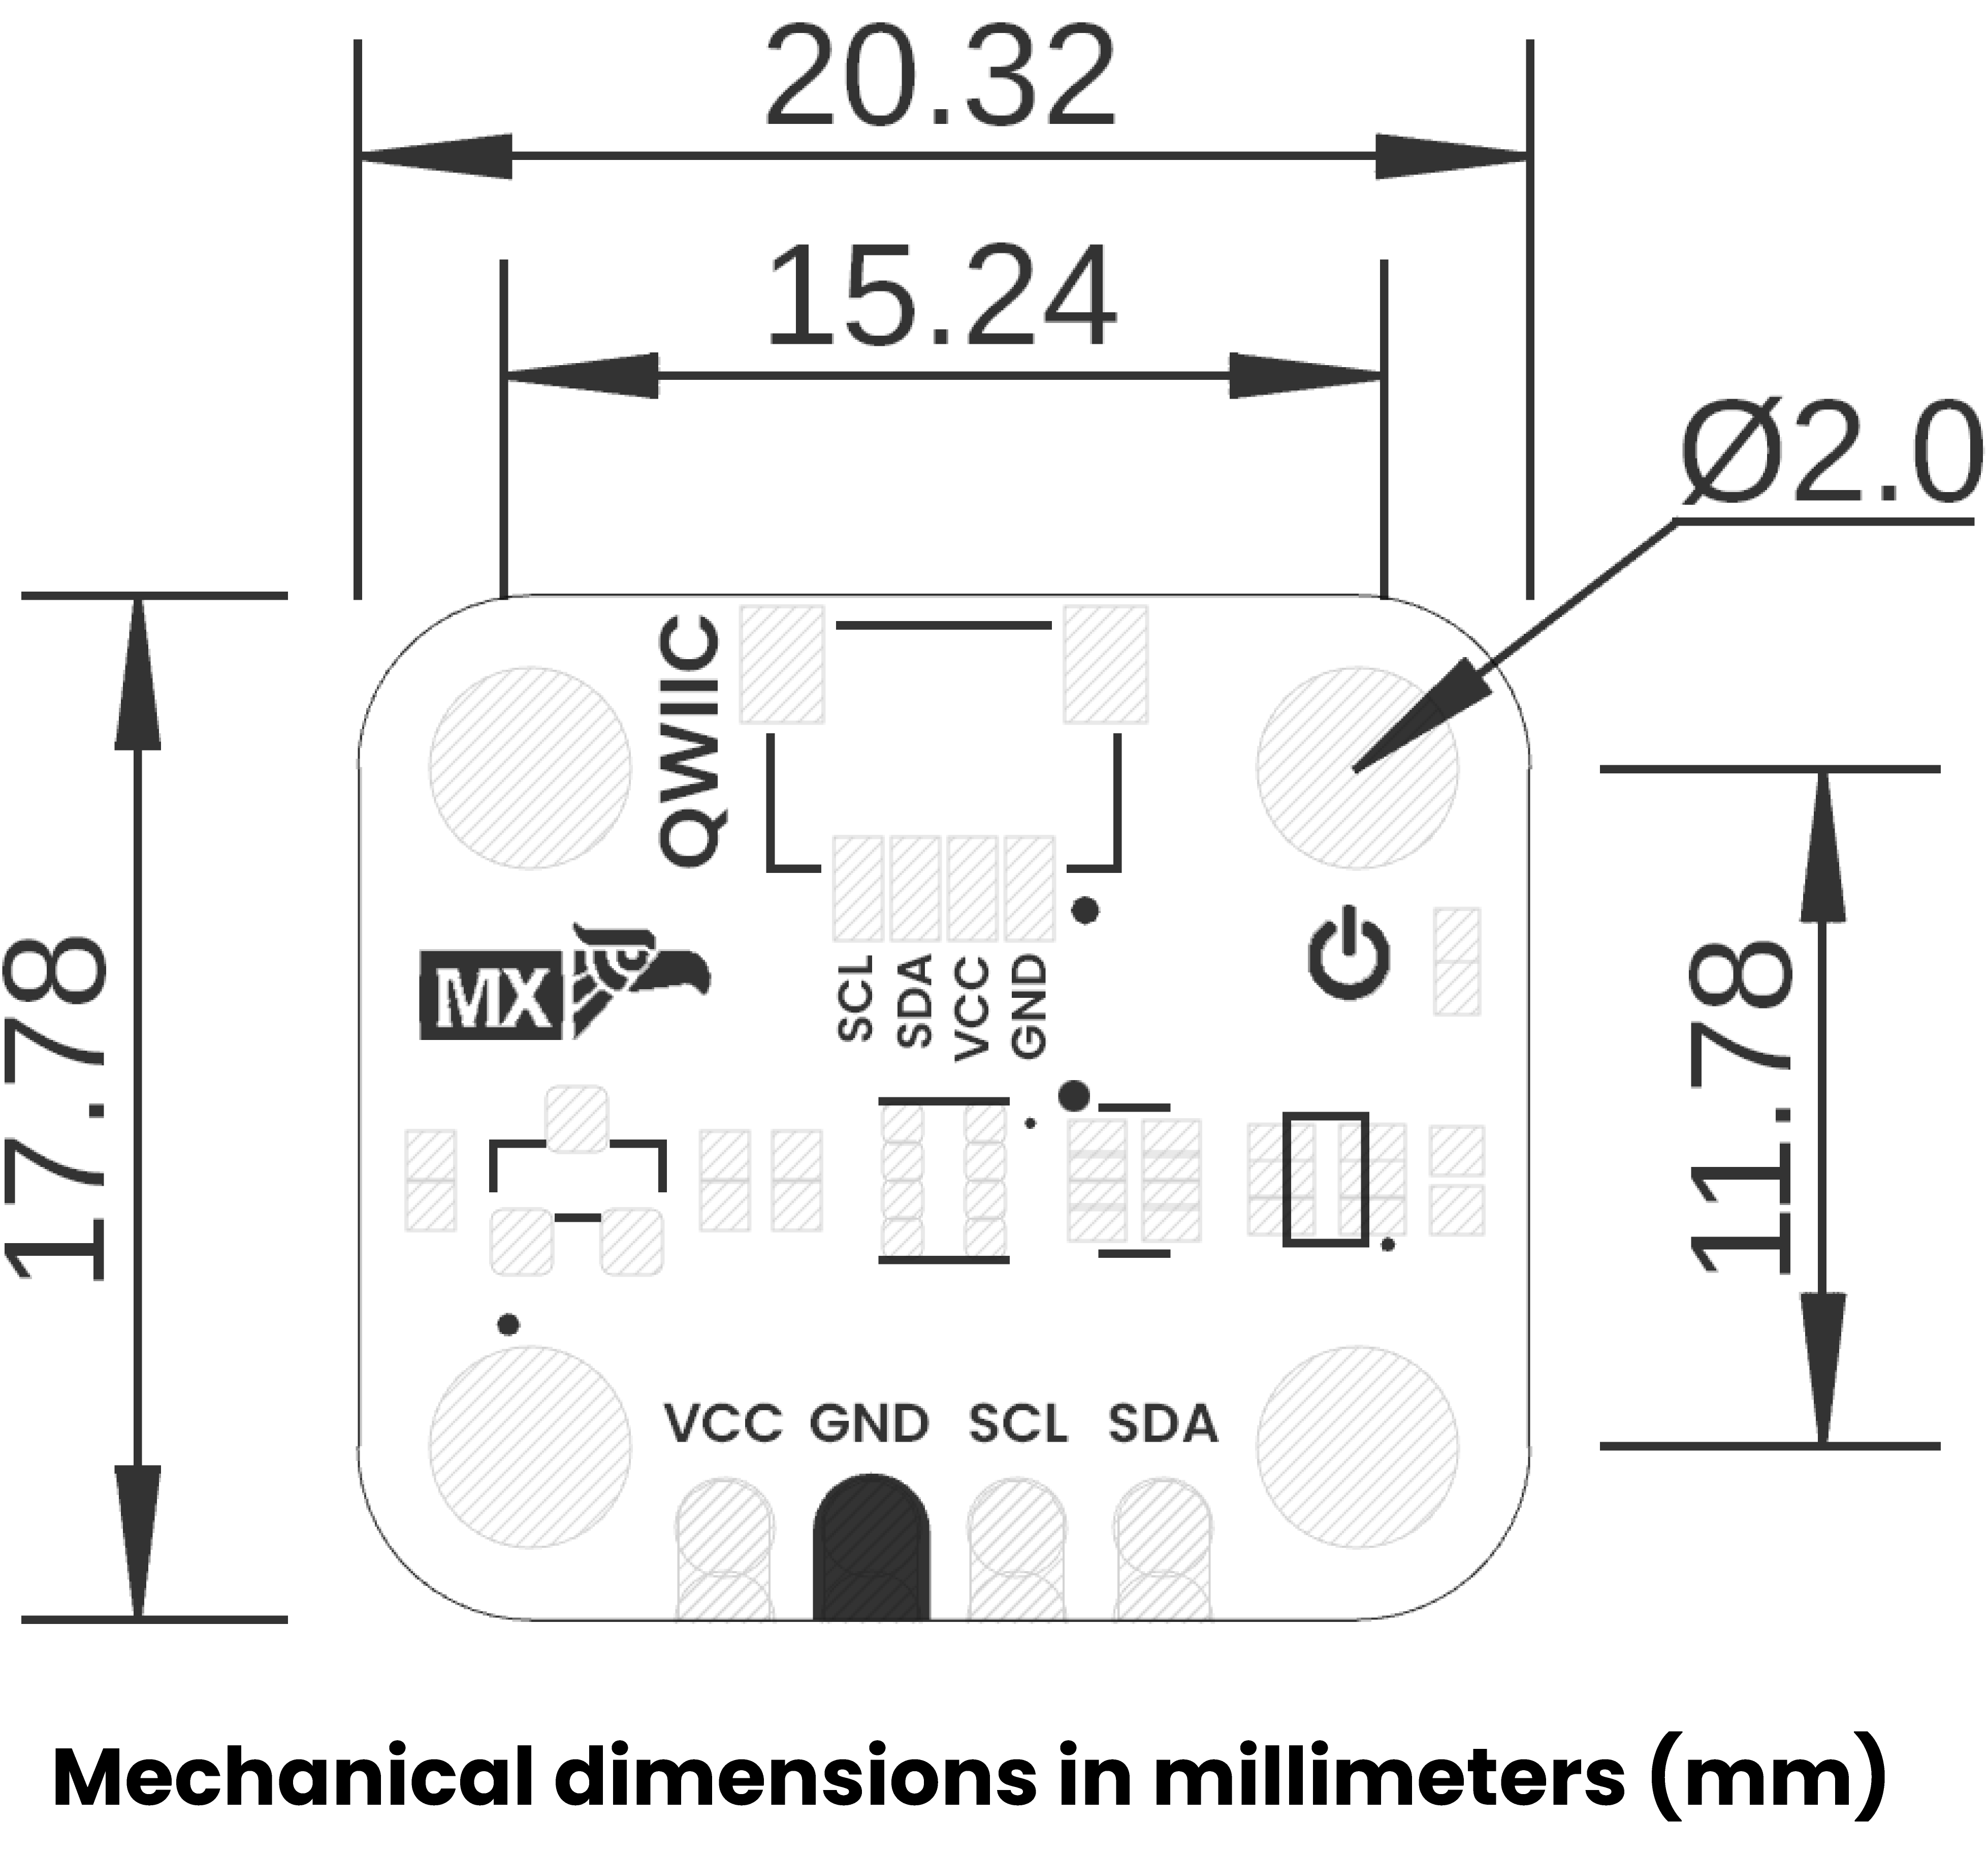
\includegraphics[width=0.6\textwidth]{es_unit_dimension_v_1_0_0_icp10111_barometric_pressure_sensor.png}
\caption{Dimensiones Físicas}
\label{fig:es-unit-dimension-v-1-0-0-icp10111-barometric-pressure-sensor-png}
\end{figure}




\begin{figure}[H]
\centering
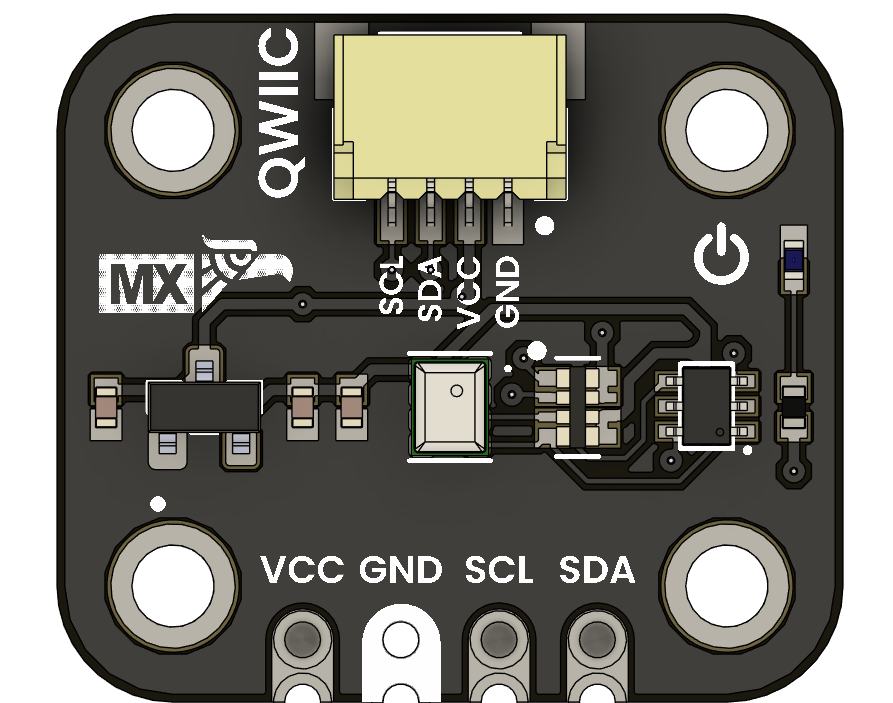
\includegraphics[width=0.7\textwidth]{es_unit_top_v_1_0_0_icp10111_barometric_pressure_sensor.png}
\caption{Vista Superior}
\label{fig:es-unit-top-v-1-0-0-icp10111-barometric-pressure-sensor-png}
\end{figure}




\begin{figure}[H]
\centering
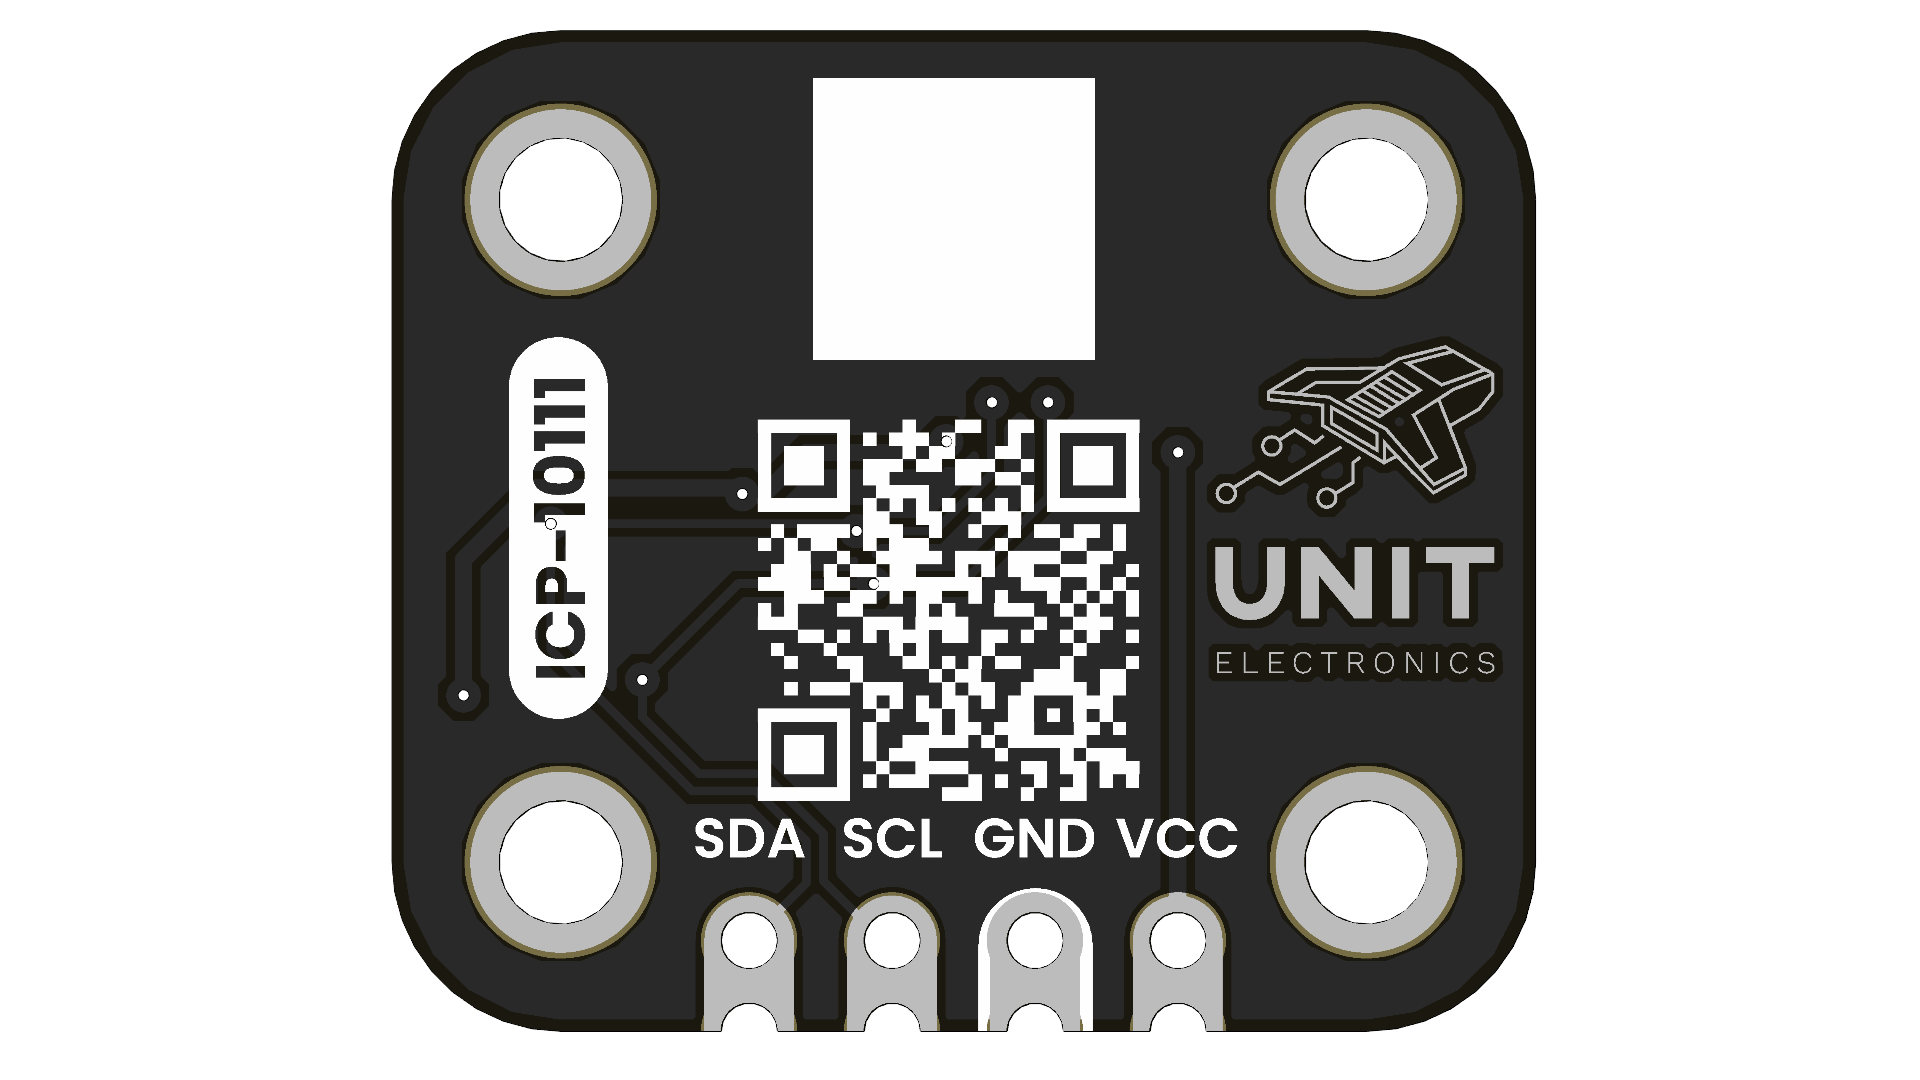
\includegraphics[width=0.7\textwidth]{es_unit_btm_v_1_0_0_icp10111_barometric_pressure_sensor.png}
\caption{Vista Inferior}
\label{fig:es-unit-btm-v-1-0-0-icp10111-barometric-pressure-sensor-png}
\end{figure}



\subsubsection{Información del Encapsulado}


\begin{table}[H]
\centering
\small
\begin{tabular}{|c|c|c|}
\hline
Parámetro & Valor & Unidad \\
\hline
Tipo de Encapsulado & QFN-48 & - \\
Dimensiones & 6 x 6 x 0.9 & mm \\
Separación de Pines & 0.4 & mm \\
Peso & 0.5 & g \\
\hline
\end{tabular}
\caption{Especificaciones técnicas}
\end{table}


\subsubsection{Especificaciones Ambientales}


\begin{table}[H]
\centering
\small
\begin{tabular}{|l|l|l|l|l|}
\hline
Parámetro & Mín & Máx & Unidad & Condiciones \\
\hline
Temperatura de Operación & -40 & +85 & $^{\circ}$C & Grado comercial \\
Temperatura de Almacenamiento & -55 & +125 & $^{\circ}$C & - \\
Humedad & 10 & 95 & %HR & Sin condensación \\
\hline
\end{tabular}
\caption{Especificaciones técnicas}
\end{table}


\subsection{Soporte de Software}

\subsubsection{Entorno de Desarrollo}
\begin{itemize}
\item \textbf{Arduino IDE}: Soporte completo con núcleo ESP32
\item \textbf{ESP-IDF}: Framework nativo de Espressif
\item \textbf{PlatformIO}: Soporte IDE multiplataforma
\item \textbf{MicroPython}: Soporte Python para desarrollo rápido
\end{itemize}

\subsubsection{Librerías Principales}
\begin{itemize}
\item Conectividad WiFi & Bluetooth
\item Sistema operativo en tiempo real FreeRTOS
\item Capa de abstracción de hardware (HAL)
\item Soporte de actualización por aire (OTA)
\end{itemize}

\subsection{Aplicaciones}

El módulo DevLab es ideal para:

\begin{enumerate}
\item \textbf{Sensores y Actuadores IoT}
\end{enumerate}
\begin{itemize}
\item Monitoreo ambiental
\item Dispositivos domóticos
\item Automatización industrial
\end{itemize}

\begin{enumerate}
\item \textbf{Prototipado y Desarrollo}
\end{enumerate}
\begin{itemize}
\item Pruebas de concepto rápidas
\item Proyectos educativos
\item Aplicaciones de investigación
\end{itemize}

\begin{enumerate}
\item \textbf{Productos Comerciales}
\end{enumerate}
\begin{itemize}
\item Electrodomésticos inteligentes
\item Dispositivos vestibles
\item Iluminación conectada
\end{itemize}

\subsection{Seguridad y Cumplimiento}

\subsubsection{Certificaciones}
\begin{itemize}
\item \textbf{FCC}: Parte 15.247 (USA)
\item \textbf{CE}: EN 300 328, EN 301 489 (Europa)
\item \textbf{IC}: RSS-210 (Canadá)
\end{itemize}

\subsubsection{Características de Seguridad}
\begin{itemize}
\item \textbf{Protección ESD}: $\pm$2kV HBM en todos los pines
\item \textbf{Inmunidad Latch-up}: $\pm$100mA
\item \textbf{Protección Térmica}: Apagado térmico automático
\end{itemize}

\subsection{Información de Pedidos}


\begin{table}[H]
\centering
\small
\begin{tabular}{|l|l|l|l|}
\hline
Número de Parte & Descripción & Empaque & MOQ \\
\hline
DEVLAB-001 & Módulo Estándar & Bandeja & 100 \\
DEVLAB-001R & Compatible RoHS & Tape & Reel & 1000 \\
DEVLAB-DEV & Kit de Desarrollo & Caja Individual & 1 \\
\hline
\end{tabular}
\caption{Especificaciones técnicas}
\end{table}


\subsection{Historial de Revisiones}


\begin{table}[H]
\centering
\small
\begin{tabular}{|c|c|c|}
\hline
Versión & Fecha & Cambios \\
\hline
1.0 & 2025-07-18 & Lanzamiento inicial \\
\hline
\end{tabular}
\caption{Especificaciones técnicas}
\end{table}


\subsection{Esquemáticos}


\begin{figure}[H]
\centering
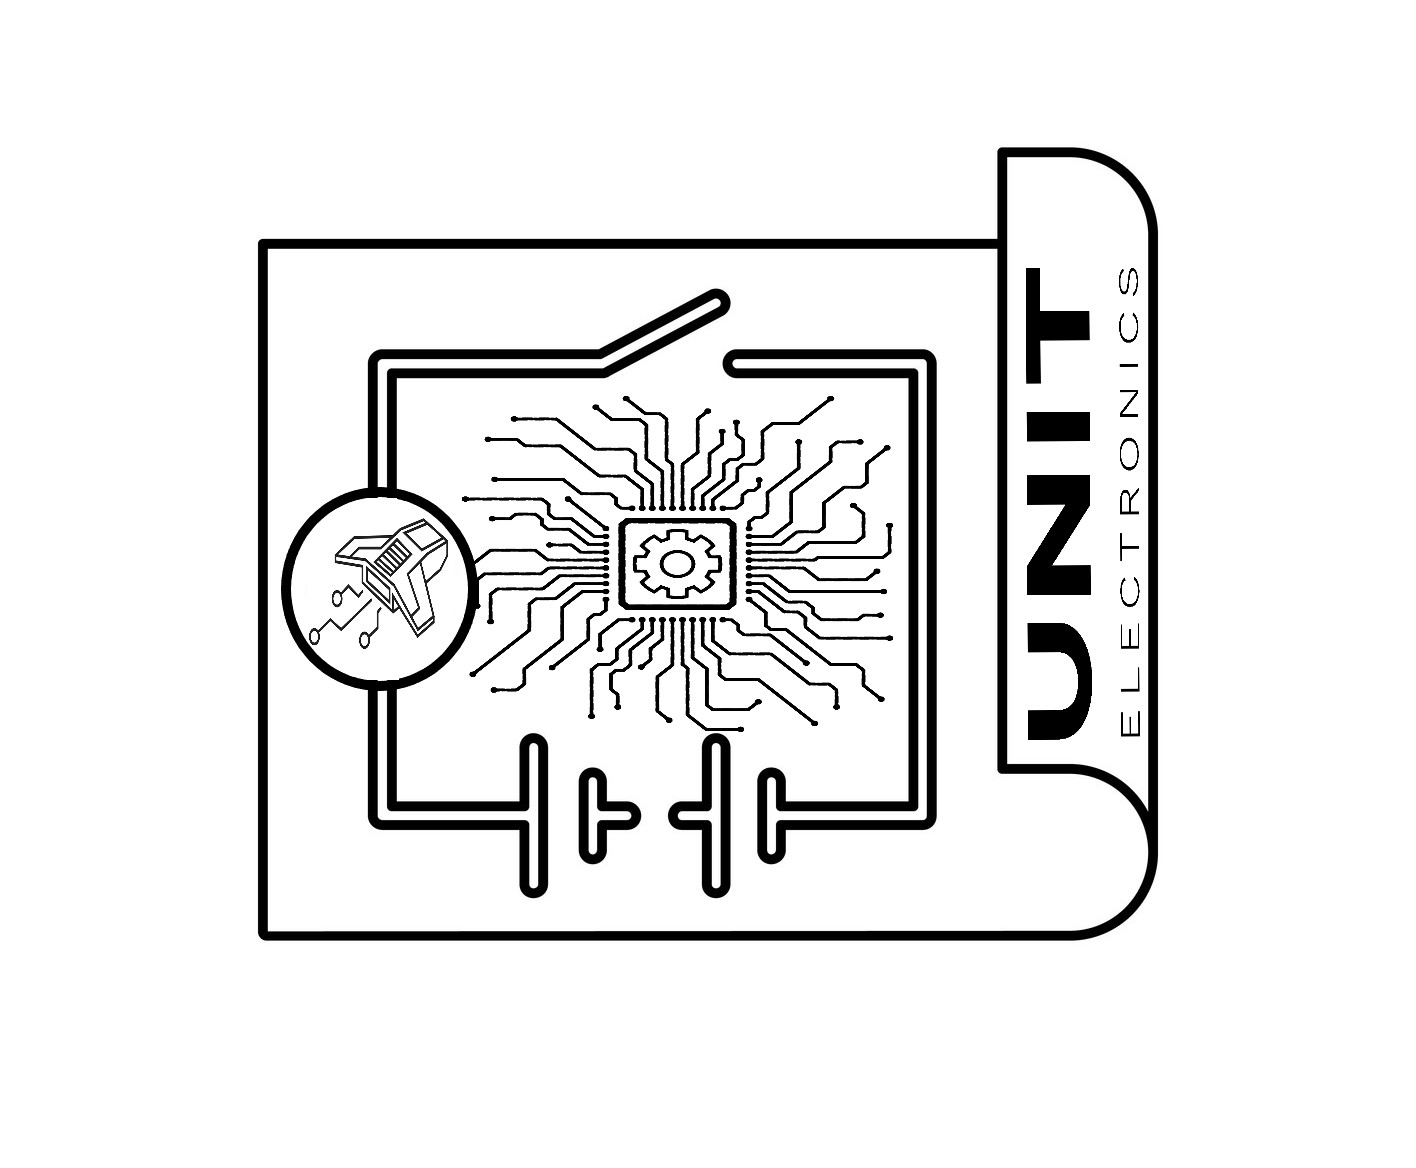
\includegraphics[width=\textwidth]{es_Schematics_icon.jpg}
\caption{Esquemático del Circuito}
\label{fig:es-Schematics-icon-jpg}
\end{figure}



---

\textit{Para soporte técnico e información adicional, visita nuestro sitio web o contacta a nuestro equipo de ingeniería.}


\end{document}
